
\thispagestyle{empty}
\begin{center}
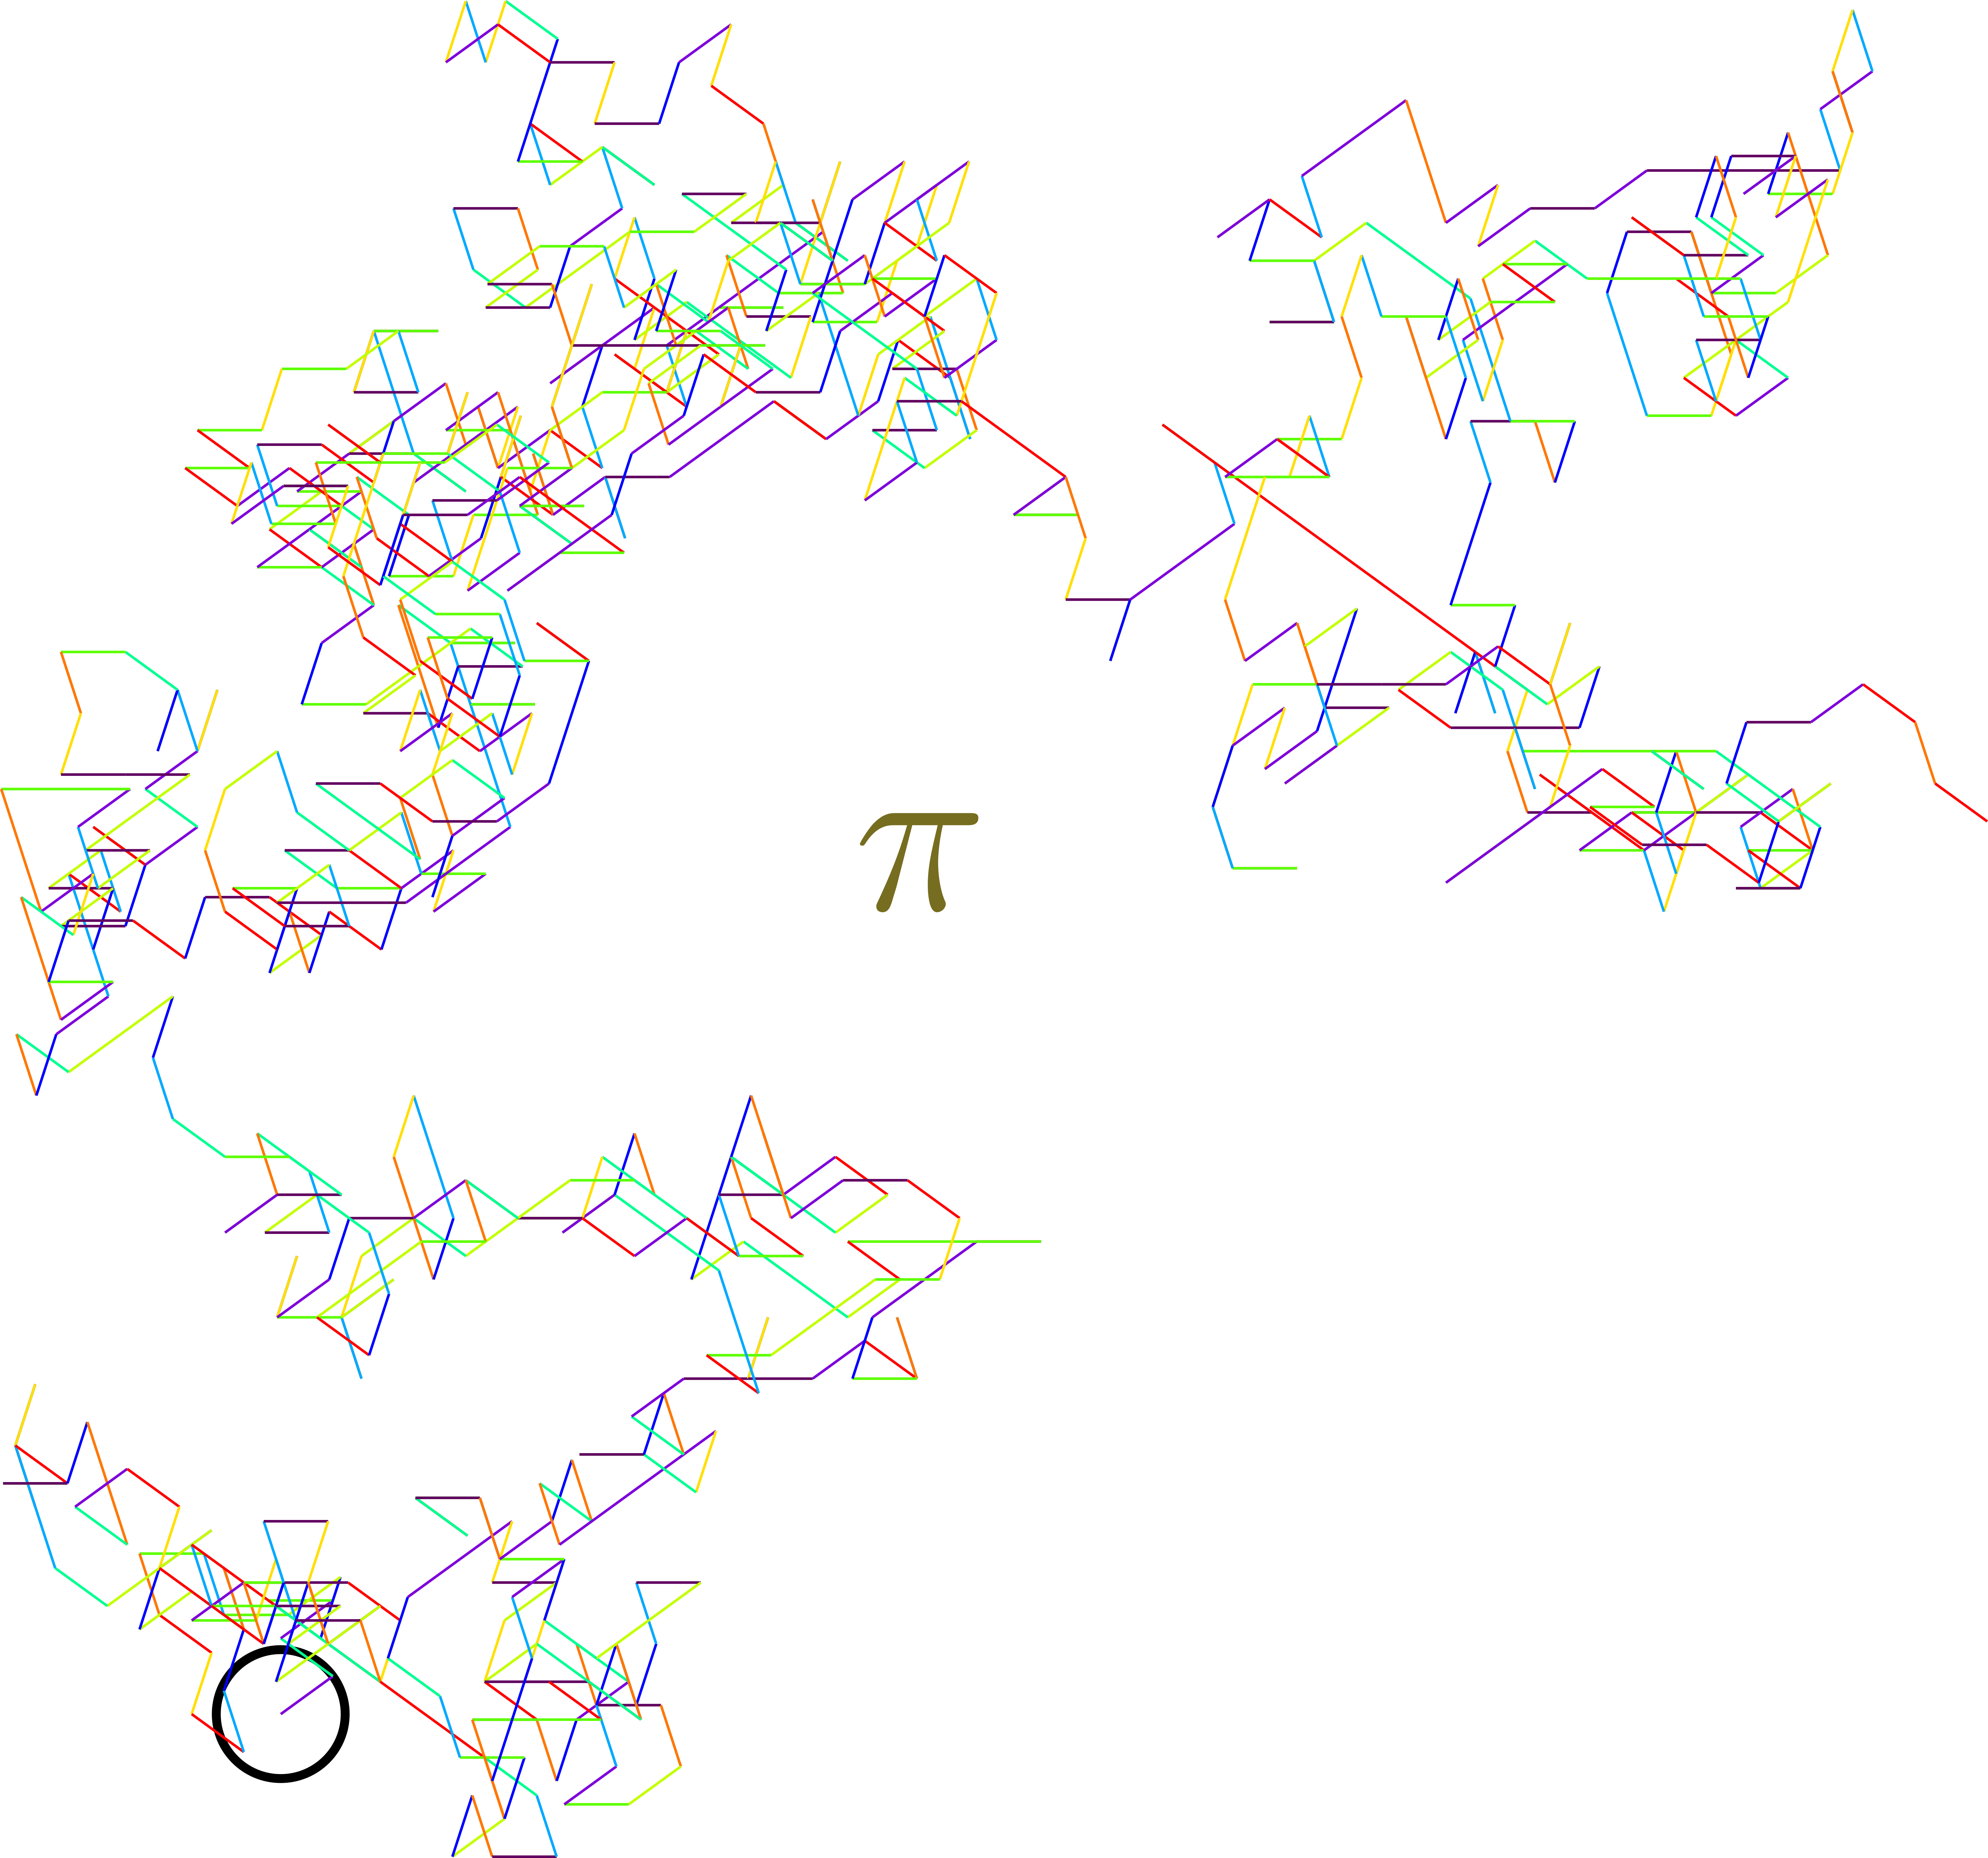
\includegraphics[width=\textwidth]{./bilder/pi.png}
\end{center}
\vspace*{\fill}
%{\Huge\color{farbe}\hfill{\ttfamily{Fangen}}}
{\centering\fontsize{50}{48} \color{farbe}\sffamily{Zahlen und Ziffern}\par}
\addcontentsline{toc}{chapter}{Zahlen und Ziffern}
\newpage
%%%%%%%%%%%%%%%%%%%%%%%%%%%%%%%%%%%%%%%%%%%%%%%%%%%%%%%%%%%%%%%%%%%%%%%%%%%%%%%
\lettrine[lines=3, lhang=.2, loversize=.25, lraise=0.05, findent=0.1em,nindent=0em]{A}{ls} wir die Geschichte \enquote{Acht} in diesem Buch geschrieben haben, haben wir anstelle von Namen Ziffern verwendet. Ein wie ich finde hübscher Einfall von Paula, der prima funktioniert. Aber warum tut er das? Warum ist es möglich, dass sofort klar ist, dass das Zeichen \Circled{8} etwas wie ein Name sein soll? Die Antwort ist, dass wir hier mit dem Unterschied zwischen Ziffern und Zahlen gespielt haben. Wenn Du 8 liest, hast du etwas sehr Kompliziertes im Kopf, etwas, wofür die Menschheit sehr lange gebraucht hat, es zu verstehen: eine Zahl. Mittlerweile können Mathematikerinnen zwar erklären, was eine Zahl ist, das ist aber sehr verwirrend und kompliziert.

Zahlen haben nichts damit zu tun, wie man sie schreibt oder darstellt. Da haben verschiedene Kulturen verschiedene Lösungen gefunden, die mal mehr und mal weniger tauglich sind, Schülerinnen das Rechnen beizubringen. Ein paar davon möchte ich dir hier vorstellen.

Aber vorher nochmals zurück zu den Zahlen. Zahlen sind universell, das heisst, die Regeln, denen sie folgen gelten überall und immer. Warum weiss niemand, aber das Wort \enquote{universell} darfst du wörtlich verstehen. Wenn es Ausserirdische geben sollte --wovon ich übrigens auch aus rein mathematischen Überlegungen ausgehe-- und wir irgendwann einmal Kontakt mit ihnen haben, sollte unsere Mathematik und die der Ausserirdischen dieselbe sein, auch wenn sie sonst vielleicht mit Lichtblitzen statt mit Schallwellen kommunizieren.

Das gilt auch auf der Erde. Egal welche Sprache du sprichst, Mathematik funktioniert immer. Nicht, dass irgendjemand die gesamte Mathematik versteht, aber es sollte möglich sein, jemanden zu finden, der intelligent genug ist, den Bereich zu verstehen und zu beweisen, ob das was mit Mathematik gesagt wurde, richtig ist oder falsch. Ganz präzise.

Ein Beispiel für Mathematik. Die folgenden Überlegungen sind ganz unabhängig von den Ziffern. Du spielst mit Legosteinen, alle sehen gleich aus und bestehen aus zwei Reihen mit je vier von diesen Noppen\footnote{Dieser 4x2 Stein ist übrigens der klassischste aller Legosteine. Er ist massstäblich einem echten Backstein nachempfunden. Alle anderen Legosteine leiten ihre Grösse genau von diesem Stein ab.}. Und Du hast jetzt ein paar Steine davon und willst wissen, wie viele mögliche Figuren du damit bauen kannst, das heisst du fragst dich, auf wie viele verschiedene Arten du die Steine verbinden kannst. Natürlich werden nicht alle Kombinationen schön aussehen, aber vielleicht interessiert dich doch die Frage, wie viele Dinge du mit deinen Steinen bauen könntest.

Dann hilft dir Mathematik und die gilt, egal ob du eigentlich Schweizerdeutsch, Französisch oder $!$X\'{o}\~{o} sprichst\footnote{Die Sprache ǃ X\'{o}\~{o} heisst tatsächlich so! Sie wird auch Taa genannt und gehört zu den Tuu Sprachen. Sie wird in Botswana und Namibia gesprochen, allerdings nur noch von sehr wenigen Menschen. Das Besondere ist, dass sie sehr viele Laute enthält, insgesamt 159. Man bräuchte also 159 verschiedene Buchstaben oder Buchstabenkombinationen wie im Deutschen \textit{sch} um alle Laute zu schreiben. Such mal im Internet nach der Sprache. 83 Laute sind Schnalz- und Klicklaute. Für unsere Ohren klingt das sehr spannend!}. Aber wie so oft üblich, müssen wir erst einmal eine Einschränkung machen. Wir sehen uns nur Kombinationen an, bei der die Steine entweder parallel oder im rechten Winkel zueinander sind. Steine \textit{schief} aneinander zu bauen, ist nicht erlaubt, dann wäre die Lösung schon bei zwei Steinen unendlich. Die Formel zu Berechnung der Anzahl möglicher Kombinationen lautet:

$$2^{n-1}+\frac{46^{n-1}-2^{n-1}}{2}$$

Oha! Wer soll denn das verstehen? Aber es ist weniger schwierig las du denkst, lass dich von der Schreibweise nicht abschrecken! Rechnen wir es doch mal an einem Beispiel durch. Sagen wir, du hast nur zwei Steine zur Verfügung. überleg erst einmal selbst im Kopf, wie du beide Steine kombinieren kannst.

Und jetzt lass uns kurz rechnen. $n$ ist die Anzahl der Steine, die du zur Verfügung hast. Im Beispiel gilt also $n=2$. Jetzt setzen wir die 2 in die Gleichung ein. Wie du vielleicht schon aus der Schule weisst, bedeutet die Schreibweise, wenn etwas hochgestellt ist, auch \textit{hoch} oder besser ausgedrückt, Potenz. $2^3$ heisst nichts anderes, als dass wir $2\times2\times2$ rechnen. Probieren wir das doch mal mit dem ersten Stück (Term genannt) der Gleichung aus und rechnen $2^{2-1}=2^1=2$ Okay. Dazu addieren wir den zweiten Term, den wir stückweise ausrechnen. Beginnen wir über dem Bruchstrich. $46^{2-1}=46$. Davon ziehen wir wieder die bereits bekannten $2^{2-1}=2$ ab und kommen auf 44. Der Bruchstrich ist nichts anderes als ein \textit{geteilt durch das was unten steht}, also $2$. Die Lösung für zwei Steine ist, dass es $24$ verschiedene Kombinationen gibt.

Das verrückte an dieser Formel ist, die Lösung wächst unglaublich schnell, das bedeutet, dass die Anzahl möglicher Kombinationen sehr schnell sehr gross wird, wenn du nur wenige Steine hinzunimmst. Die Anzahl Kombinationen beträgt zum Beispiel für 6 legosteine $915'103’765$ also fast eine Milliarde. Probiere es aus, wenn du es nicht glaubst! Wenn Du allerdings je Kombination sagen wir 10 Sekunden benötigst, wirst du 290 Jahre Tag und Nacht beschäftigt sein. Eine langweilige Idee, nehme ich an. Bei 25 Steinen beträgt die Anzahl Kombinationen

\begin{footnotesize}
$$4'028'635'400'867'168'454'517'798'790'018'457'665’536$$
\end{footnotesize}

Eine bizarr grosse Zahl! Viel mehr weiss man nicht, die Zahlen, die danach folgen, sind schlicht zu gross, um berechnet zu werden. Für 47 Lego-Steine bräuchte der beste Computer (Stand 2005) 130 Jahre. Nein halt, ganz falsch, er bräuchte eine Anzahl Jahre, bei der auf die 130 noch 39 Nullen folgen! Keine Chance in diesem Universum.

So kann man also verschiedenste Dinge mit Hilfe der Mathematik beschreiben und verstehen. Mit Mathematik könnten wir uns also auch mit Ausserirdischen über Lego unterhalten. Würde mich doch sehr wundern, wenn die nicht etwas Ähnliches bei sich haben. Aber es gibt auch einen Teil, der eben nicht gleich ist auf der Welt und das sind die Ziffern. Ziffern ist die Art, wie du Zahlen schreibst, welche Zeichen und welches System du verwendest. Mit System meine ich übrigens den logischen Aufbau der Ziffern, dazu komme ich gleich noch.

Die Unterschiede zwischen den Kulturen betreffen nicht nur die Art, wie die Ziffern geschrieben werden, sondern auch, wie sie benannt werden. Damit meine ich nicht den reinen Wortlaut wie \textit{zwei} auf Hochdeutsch, \textit{two} auf Englisch oder \textit{$\neq$n\^{u}m} auf $!$X\'{o}\~{o}. Wie man das Zeichen $\neq$ wohl auspricht? --sondern wie die Wörter für die Zahlen aufgebaut sind. Jetzt kommt etwas sehr Kompliziertes, das du vermutlich noch nicht verstehst. Mathematik beschäftigt sich mit dem Wert der Zahlen. Und dabei spielt es keine Rolle, wie die Zahlen geschrieben oder benannt werden. Das wird durch die Kultur und gelegentlich praktischen Gründen bestimmt.

Wir verwenden indisch-arabischen Ziffern, die haben sich in Indien aus der Brahmi-Schrift (3. Jahrhundert vor Christus, aber die Angaben gehen auseinander) entwickelt. Das betrifft weniger die Zeichen selbst, aber auch, sondern vor allem das System. Als endgültige Geburtsstunde gilt jedenfalls das Jahr 628, als ein Mann namens Brahmagupta die Null als vollwertige Zahl etabliert hatte. Da das System ziemlich gut funktioniert hat, hat es sich von da ab schnell ausgebreitet und auch die arabische Welt erreicht, die es über den Umweg Nordafrika auch in Europa populär gemacht haben. Das war dan naber erst im 13. Jahrhundert.

Aber was fanden denn die Leute damals so cool an dem System? Es verwendet nur zehn Zeichen (Glyphen ist das Angeberwort dazu) und ist streng logisch aufgebaut. Das System funktioniert nämlich ganz einfach: wenn du immer grössere Zahlen schreiben willst, fängst du zunächst mit den zehn einfachen Zeichen:

$$0, 1, 2, 3, 4, 5, 6, 7, 8, 9$$
Du musst dir nur zehn Zeichen merken und ihre Reihenfolge. Aber ab Zehn gehen dir die Zeichen aus, und du willst keine neuen hinzunehmen (weil das sonst nicht cool wäre, habe ich ja gerade gesagt). Aber funktionieren würde es schon. Man könnte ja zum Beispiel sagen, dass $\Theta$ Elf, $\Xi$ Zwölf und so weiter bedeuten könnte und so könnten wir uns für jede Zahl ein eigenes Zeichen ausdenken. Das ist aber nicht nur für dich schwer zu merken, gerade wenn du manche Zahlen nur selten benutzt, wie die wirklich blöde siebenundachtzig. Also belässt du es bei den zehn Zeichen und wendest einen genialen Trick an. Sobald dir die Zeichen ausgehen, setzten du beginnend mit dem kleinsten Zeichen nach der 0 dieses vorne dran und beginnst hinten wieder von vorne von unten nach oben die bekannten Zeichen zu verwenden. Nach $\dots, 8, 9,\dots$ kommt der Sprung $\dots, 10, 12, 13, 14,\dots$

Und wenn du dann wieder ans Ende gekommen bist, nimmst du vorne das nächste Zeichen und fängst da an hochzuzählen: $\dots, 18, 19$ und dann Zack $20, 21, 22,\dots$ und wenn dir dann wieder die Zeichen ausgehen, setzen du wieder eine Ziffer vorne dran, nach $\dots, 98, 99$ geht es weiter mit $100, 101,102\dots$. Alles sehr schön logisch und unkompliziert. Damit kannst du leicht und verständlich beliebig grosse Zahlen schreiben.

Und dann hat diese Schreibweise den Vorteil, dass sie sogar noch leicht erweiterbar ist, wenn du nämlich Zahlen schreiben willst (oder eher musst) die zum Beispiel grösser als $1$, aber kleiner als $2$ sind. Dann setzt man nämlich ein Komma (oder wie hier in der Schweiz und vielen anderen Ländern üblich einen Punkt) hinter die letzte volle Zahl und kann dann den sogenannten gebrochenen Teil weiterschreiben. Versuch mal da mit eigenen Worten zu erklären, wie die Regel funktioniert und warum zum Beispiel $4.5$ grösser ist als $4.42$.

Die verwendeten Zeichen können sich natürlich je nach Schrift unterscheiden, das System bleibt aber in den meisten Sprachen dasselbe. Hier ein paar, die mir gefallen (manchmal steht an der Stelle der Null das Zeichen für 10):

\begin{center}
\small
\begin{tabular}{ c c c c c c c c c c l}
0 & 1 & 2 & 3 & 4 & 5 & 6 & 7 & 8 & 9 & {\tiny Hindu-Arabisch}\\
\FontC{௦} & \FontC{௧} & \FontC{௨} & \FontC{௩} & \FontC{௪} & \FontC{௫} & \FontC{௬} & \FontC{௭} & \FontC{௮} & \FontC{௯} & {\tiny Tamil}\\
\FontD{0} & \FontD{๑} & \FontD{๒} & \FontD{๓} & \FontD{๔} & \FontD{๕} & \FontD{๖} & \FontD{๗} & \FontD{๘} & \FontD{๙} & {\tiny Thai}\\
\FontE{ი} & \FontE{ა} & \FontE{ბ} & \FontE{გ} & \FontE{დ} & \FontE{ე} & \FontE{ვ} & \FontE{ზ} & \FontE{ჱ} & \FontE{თ} & {\tiny Georgisch}\\
\FontF{०} & \FontF{१} & \FontF{२} & \FontF{३} & \FontF{४} & \FontF{५} & \FontF{६} & \FontF{७} & \FontF{८} & \FontF{९} & {\tiny Devanagari}\\
\FontG{十} & \FontG{一} & \FontG{二} & \FontG{三} & \FontG{四} & \FontG{五} & \FontG{六} & \FontG{七} & \FontG{八} & \FontG{九} & {\tiny Japanisch}\\
\FontB{י} & \FontB{א} & \FontB{ב} & \FontB{ג} & \FontB{ד} & \FontB{ה} & \FontB{ו} & \FontB{ז} & \FontB{ח} & \FontB{ט} & {\tiny Hebräisch}\\
\FontH{٠} & \FontH{١} & \FontH{٢} & \FontH{٣} & \FontH{٤} & \FontH{٥} & \FontH{٦} & \FontH{٧} & \FontH{٨} & \FontH{٩} & {\tiny Arabisch}\\
\FontI{ꊰ} &\FontI{ꋍ} & \FontI{ꑍ} & \FontI{ꌕ} & \FontI{ꇖ} & \FontI{ꉬ} & \FontI{ꃘ} & \FontI{ꏃ} & \FontI{ꉆ} & \FontI{ꈞ} & {\tiny Yi}\\
\end{tabular}
\end{center}
Die Mathematik hat sich seit Erfindung dieses Systems immer weiterentwickelt und wie die meisten Wissenschaften in den letzten wenigen hundert Jahren rasant. Das hat es nötig gemacht, die Schreibung von Zahlen auf viele Arten zu erweitern. Beispielsweise ist schon ganz früh klar gewesen, dass sich ein Drittel nicht ohne weiteres mit diesem System schreiben lässt, da müsstest du unendlich viele Dreien schreiben, womit du spätestens aufhören müsstest, wenn jemand \enquote{Zähneputzen} ruft. Schon in der Antike haben die Griechen zeigen können, dass das auch für $\sqrt{2}$ gilt. Sie gehört übrigens zur Gruppe der irrationalen Zahlen. Hinzu kamen negative Zahlen (mit einem Minus gekennzeichnet) und dann so verrückte Dinge wie irrationale Zahlen die man mit einem $i$ schreibt und manche Zahlen, die auch nicht gutgeschrieben werden können, haben dann doch noch ein eigenes Zeichen bekommen, wie die berühmte Kreiszahl $\Pi$.

Das System, Zahlen so aufzubauen, lässt sich übrigens leicht variieren. Warum zum Beispiel ausgerechnet zehn verschiedene Symbole? Na ja, die einfache Antwort ist wohl, dass die meisten Menschen zehn Finger haben und unser Zählen als Kind damit beginnt. Aber das ist nicht immer das einfachste. Ein Computer funktioniert so, dass er eigentlich nur zwischen \textit{da fliesst gerade Strom} und \textit{da fliesst gerade kein Strom} unterscheiden kann. Dann kannst du dir den Speicher des Computers ganz vereinfacht vorstellen als viele Punkte, an denen entweder eben Strom fliesst oder eben nicht. Wenn wir jetzt Strom fliesst mit dem Symbol $1$ bezeichnen und kein Strom mit $0$, können wir Zahlen in einem sogenannten Binärystem, also mit lediglich zwei Zeichen schreiben. Die Logik bleibt dieselbe:

\begin{small}
\begin{center}
\begin{tabular}{ c c l }
0 & 0 & die ersten beiden Zahlen sind noch gleich\\
1 & 1 & ab der 1 fehlen uns aber weitere Zeichen \\
2 & 10 & also fügen wir vorne wieder eine an \\
3 & 11 & unten hinter wieder weiterzählen\\
& & Ach schon wieder fertig?\\
&& Also wieder vorne eine dazu\dots \\
4 & 100 & und so weiter bis Unendlich.
\end{tabular}
\end{center}
\end{small}
Manchmal werden im Computer (auf einer anderen Eben, das ist hier aber egal) auch sogenannte Hexadezimalzahlen eingesetzt. Das System verwendet 16 verschiedene Zeichen, nach der $9$ folgt $A$, als elf dann $B$ und so weiter bis fünfzehn als $F$. Das Hexadezimalsystem wird verwendet, da man somit die Leistung des Computers optimal nutzen kann. Wieso genau sei jetzt mal egal\footnote{Ich habe zwar versucht, zu erklären warum das so ist, aber nicht geschafft, es in einfache Worte zu bringen. Da lass ich es doch einfach weg. Frag mich, wenn es dich interessiert.}. Ein anderes Beispiel ist das Zahlensystem der Maya (die früher in Mexiko gelebt haben). Sie hatten als Basis die zwanzig. Ihre Ziffern waren so aufgebaut

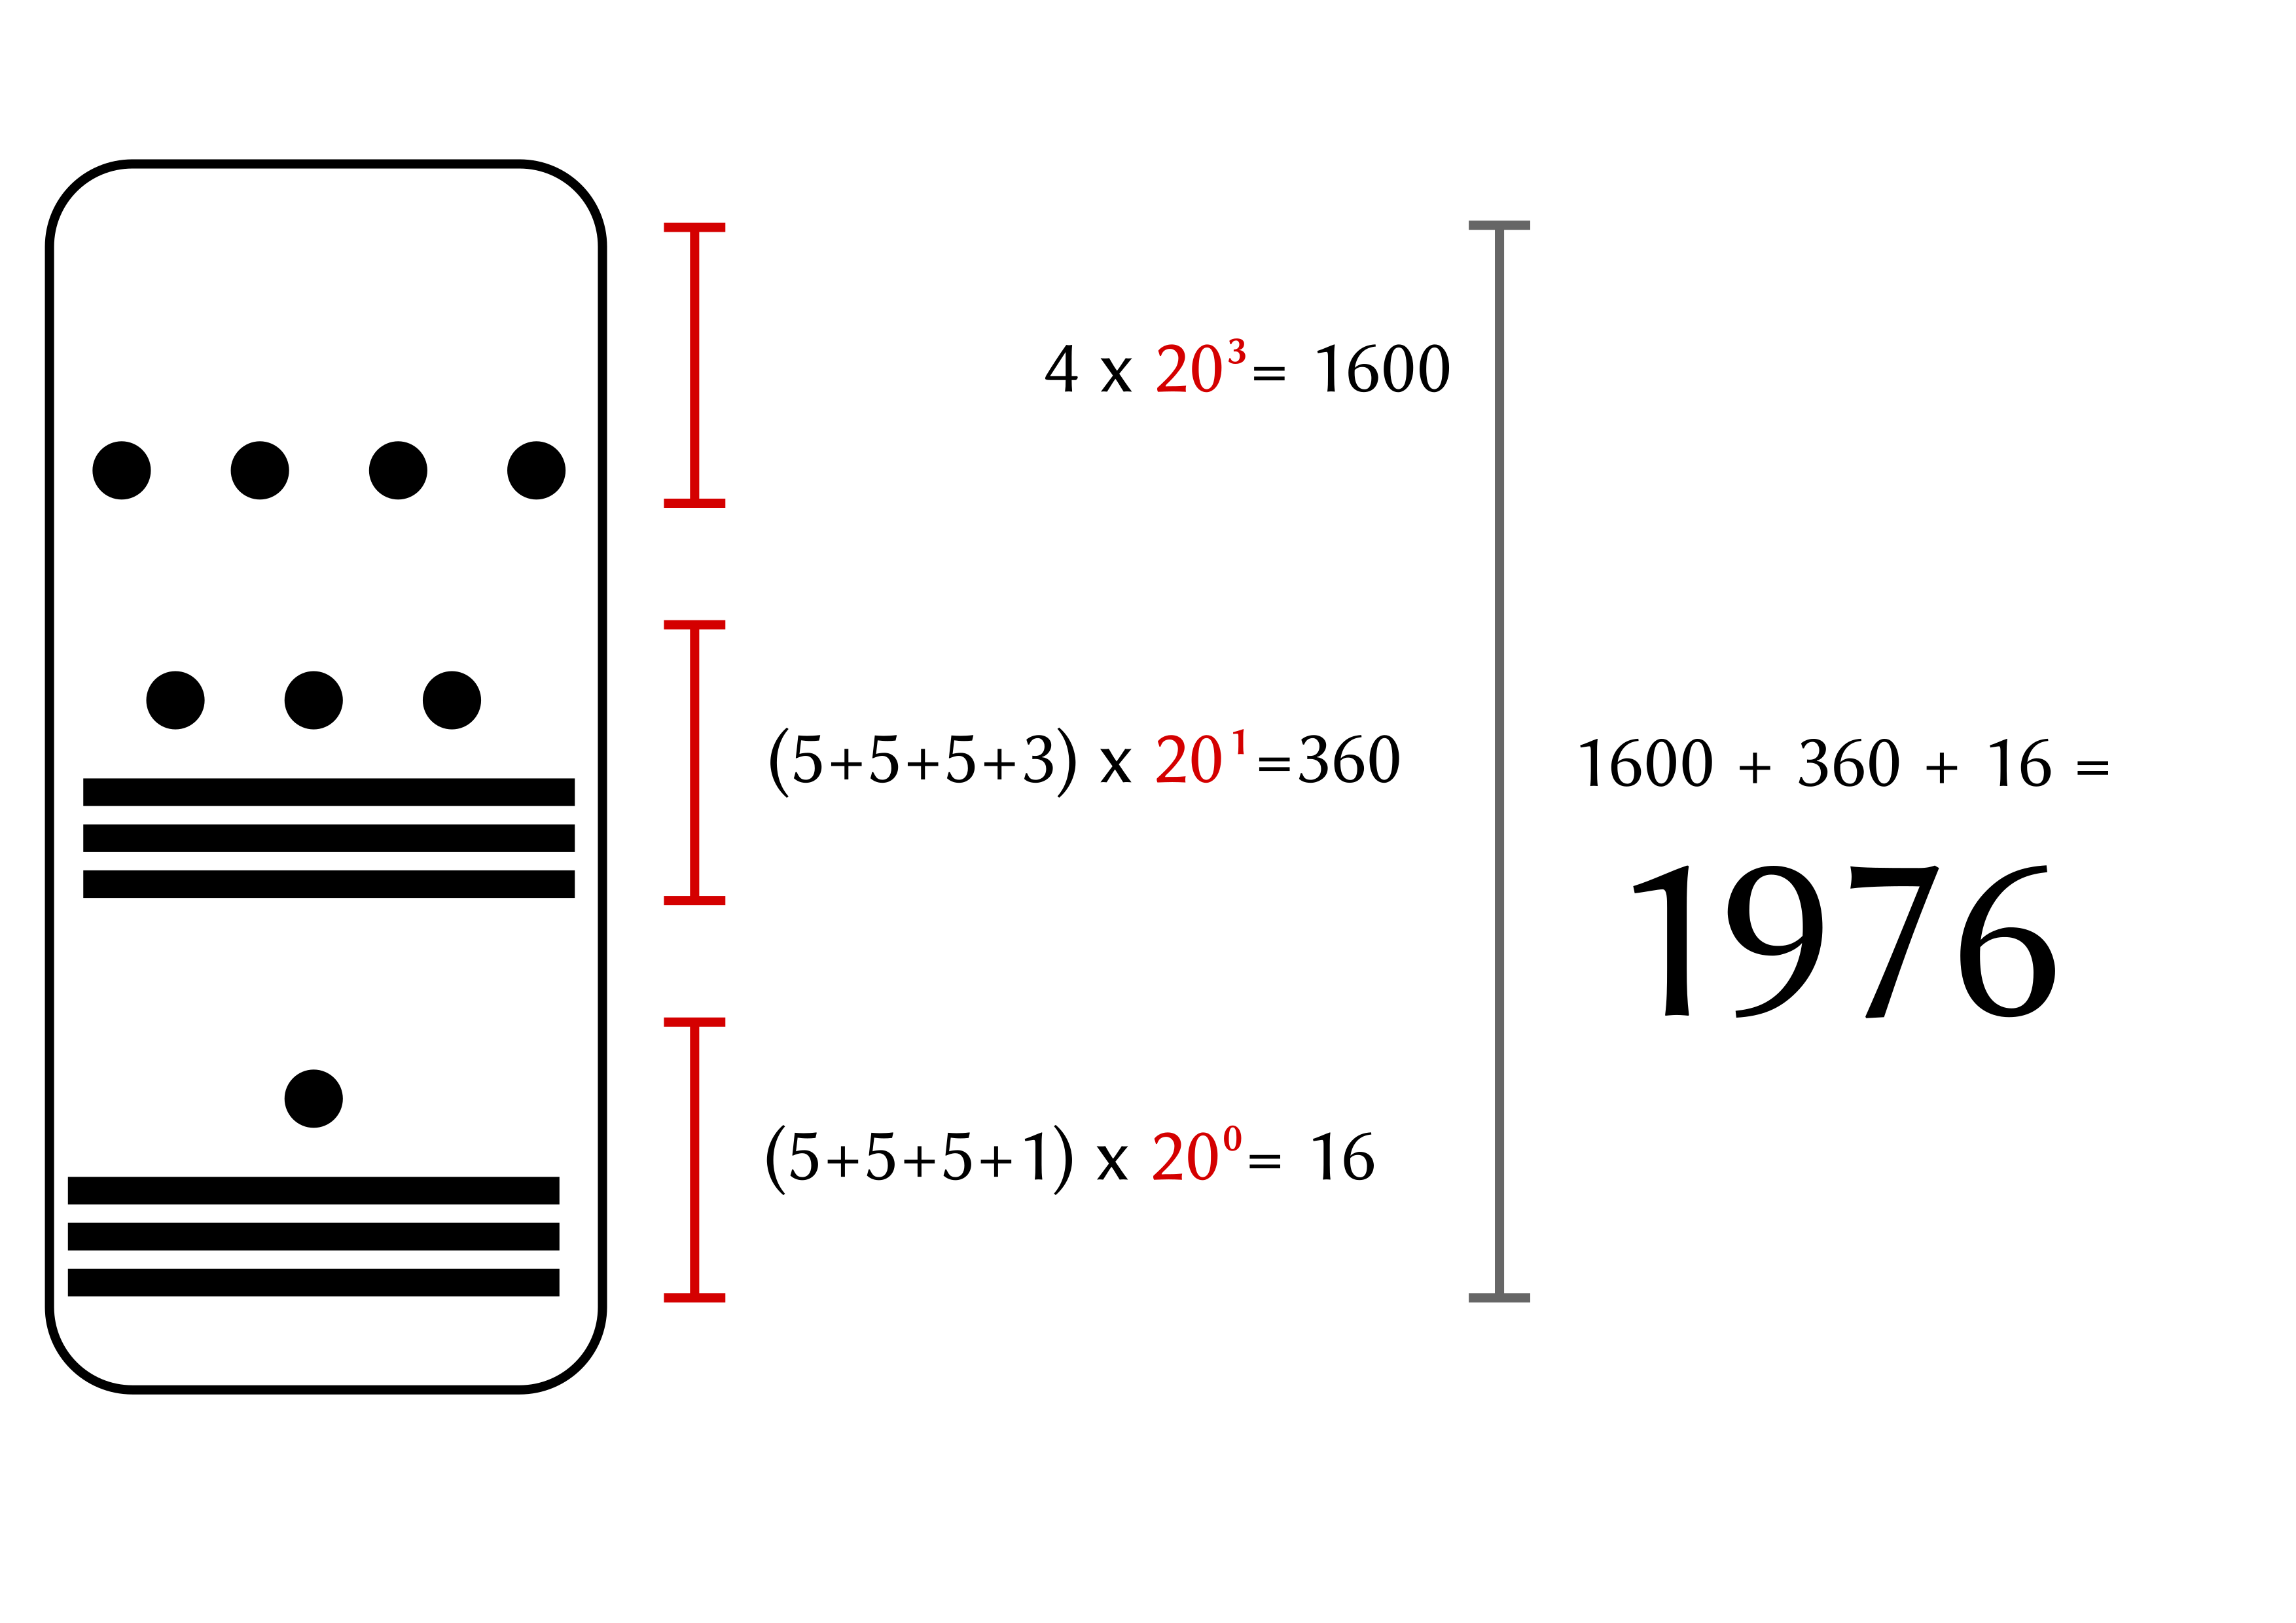
\includegraphics[width=\textwidth]{./bilder/Maya1976.png}

Und es gibt noch viel mehr Möglichkeiten, Zahlen zu schreiben, die sich aber nicht bewährt haben.

Die einfachste und erste Methode wird Unärsystem genannt und ist schon mindestens 50'000 Jahre alt. Um sich das Rechnen zu erleichtern, haben Menschen damals einfach Kerben in ein Stück Holz oder einen Knochen geritzt. Die Menschen haben also zunächst nur ein Zeichen verwendet, nämlich einen Strich |. Und dann lautet die Regel zur Bildung der Zahlen einfach, dass sie das Zeichen so oft wiederholen mussten, bis es dem gewünschten Wert entsprach. 13 schreibt man also einfach als |||||||||||||.

Das ist sehr mühsam und kann leicht zu Verwechslungen führen. Daher hat man angefangen, die Striche zu gruppieren. Aus der Bronzezeit sind zum Beispiel Ägäische Zahlzeichen überliefert. Dort sahen die ersten zehn Zahlen so aus:
%%%%%%%%%%%%%%%%%%%%%Hier einfügen

Genau wie bei dieser Schrift hat man auch im alten Ägypten gewisse Anzahlen von Strichen zusammengefasst und ein neues Zeichen (Hieroglyphe) vergeben. Insgesamt gab es sechs verschiedene:

1 \textpmhg{\Hone}, 10 \textpmhg{2}, 100 \textpmhg{3}, 1’000 \textpmhg{4}, 10’000 \textpmhg{5}, 100’000 \textpmhg{6}, 1'000’000 \textpmhg{7}. Cäsar und die anderen im alten Rom haben dann, wenn auch wesentlich später, eine ähnliche Idee gehabt. Du kennst die römischen Ziffern sicher aus einem Asterixheft. In dem lauten Tumult der Märkten damals hat man sich oft mit Zeichensprache unterhalten. Aus zwei gekreuzten Fingern für zehn, ist dann das X geworden und für fünf, der Hälfte der Zehn hat man halt auch das halbe Zeichen verwendet, das V. Aber die schlaueste Art Zahlen zu schreiben, war das nicht. Die Null zu schreiben ging zum Beispiel gar nicht und grosse Zahlen waren sehr mühsam. Aber über viele Jahrhunderte hatte man hier in Europa keine bessere Idee, bis endlich die indisch-arabischen Ziffern eingeführt wurden.

Jetzt könnte man meinen, dass wir die Zahlen auch so nennen, wie sie geschrieben werden. Bei vielen Zahlen trifft das im Deutschen zu: $17$ also siebzehn setzt sich auch sprachlich zusammen aus \textit{sieben} und \textit{zehn}. Das passt oft. Ausnahmen sind die Elf und die Zwölf. Vor allem die Zwölf war früher, als man Dinge noch auf dem Markt eingekauft hat, eine wichtige Zahl, weil sie durch so viele andere teilbar ist, nämlich der 2, 3, 4, und 6. Das geht mit 10 nicht. Weil sie so gut teilbar ist, verwenden wir sie auch noch bei der Uhrzeit bei den Stunden und als Vielfaches von fünf, also 60 bei den Minuten. Man kann so bequem ausrechnen, wie viele Minuten eine Viertelstunde hat. Und ich nehme an, weil die Zwölf so wichtig war, hat sie einen echten eigenen Namen verdient und da musste die Elf natürlich dann auch noch einen bekommen.

Wo es sprachlich leider im Deutschen dann doch etwas durcheinandergeht, sind grössere Zahlen. Zum Beispiel wird die $135’782$ als \textit{einhundert fünf und dreissig tausend sieben hundert und zwei und achtzig} ausgesprochen. Sehr blöd. Wir nennen zuerst die erste Stelle, dann die Dritte, dann die Zweite, dann die Vierte, dann die letzte und dann die Vorletzte. Wer auf so einen Unfug wohl gekommen ist?

Aber das Problem ist in anderen Sprachen noch schlimmer. Für dich am bekanntesten ist sicher Französisch. Zum Beispiel heisst 97 \textit{quatre-vingt-dix-sept} als wörtlich übersetzt \textit{Vier (mal) Zwanzig (plus) Zehn (plus) Sieben}. Ernsthaft? Noch verrückter wird es im Dänischen. Dort scheint irgendetwas gründlich schief gelaufen zu sein. Die ja eigentlich sehr häufig verwendete Zahl 50 heisst \textit{halvtredsindstyvende}, was wörtlich übersetzt \textit{(Drei minus ein Halb) mal Zwanzig} bedeutet. Schnell nachrechnen: $3-0.5=2.5$ und $2.5\times20=\dots$ Musik spielt im Hintergrund solange mein Hirn sich quält $\dots = 50$ Stimmt, bleibt aber sehr sonderbar!

Was dir vielleicht aufgefallen ist, ist das sowohl im Dänischen, wie auch im Französischen die zwanzig eine Rolle spielt. Das macht sie in vielen Kulturen. Es könnte zwei Erklärungen dafür geben: entweder werden die Zehen beim Rechnen zu den Fingern hinzugenommen, oder diese einfach umgedreht.

Dieses sogenannte Vigesimalsystem findet man in Afrika, Asien und an vielen anderen Orten. Es ist noch nicht lange her, da hat man in England 20 Schillinge zu einem Pfund zusammengefasst. Am weitesten verbreitet war das System bei den Maya im heutigen Mexiko. Ein Bild dazu hast du ja weiter oben schon gesehen. Die Maya haben Nahuatl gesprochen, eine Sprache, die es selbst heute noch gibt\footnote{Ganz unbekannt ist dir die Sprache nicht, denn Wörter wie Tomate, Schokolade und Kakao haben wir auch im Deutschen aus Nahuatl übernommen.}. In Nahuatl leiten sich die Namen der ersten fünf Zahlen von \textit{Hand} und die nächsten fünf von \textit{entgegengesetzter Hand} ab. Das Wort für zwanzig heisst in Quiché, einer anderen Maya-Sprache k‘hal, was \textit{ganzer Mensch} bedeutet, also im Sinne von mit Fingern und Zehen. In einigen ostafrikanischen Sprachen ist das auch so.

Unser Körper bestimmt unser Zahlensystem. Da wundert es mich doch, dass in der Welt der Simpsons auch ein 10er-Zahlensystem existiert, auch wenn dort alle nur vier Finger an jeder Hand haben. Wenn du dich übrigens geschickt anstellst und das Prinzip kennst, kannst du mit den Händen locker bis 59‘048 zählen. Es geht sogar noch höher, wenn du gelenkig bist. Such das mal im Internet, das Prinzip ist verblüffend. Auch heute noch wird auf manchen Märkten mit solchen Techniken gezählt, das nennt man irritierenderweise \enquote{Frauenrechnen} oder \enquote{Arithmetik aus Marseille}.

In wieder anderen Sprachen gibt es nur wenige Wörter für Zahlen. Das aus unserer Sicht wohl skurrilste Beispiel ist die Sprache der Piraha, das ist ein Volk, das im brasilianischen Amazonasgebiet lebt. Die kennen nur drei Zahlen: \textit{eins}, \textit{zwei} und \textit{viele}. Verwirrenderweise kommt noch hinzu, dass das Wort für \textit{eins} dasselbe ist wie für \textit{zwei}, bloss anders betont. Noch verwirrender ist, dass \textit{eins} auch \enquote{ungefähr eins} und zwei \enquote{nicht viele} bedeuten kann. Nicht nur, dass die keine Wörter für Zahlen haben, es fällt ihnen auch schwer, mit einer Anzahl umzugehen. In einem Test wurden ihnen eine gewisse Anzahl Früchte gegeben, zum Beispiel zehn, und sie sollten gleichviele hinzulegen oder die Anzahl mit den Fingern zeigen. Das hat bei den meisten nicht geklappt, jedenfalls nicht mehr bei mehr als drei Früchten! Es gibt also auch ein Leben ohne Zahlen, aber aus Sicht der restlichen Menschheit ist das schon sehr selten. Ich meine damit auch gar nicht, dass die Leute dort dumm sind, Zahlen und Zählen ist einfach nur kein Teil ihrer Kultur.

Was nebenbei bemerkt spannend ist, dass ähnliche Tests auch mit Tieren gemacht wurden. Wie die genau gemacht wurden, sollte man sich vielleicht nochmals ansehen, ich habe keine Ahnung, ob das wirklich stimmen kann. Jedenfalls gilt aktuell, dass Schimpanzen demnach mindestens bis neun zählen können, viele Vögel bis sieben, Ameisen bis 20 und Ratten sogar bis 24. Mit Zählen ist gemeint, dass sie die Anzahl abschätzen können, sie haben natürlich kein Wort oder hübsches Zeichen dafür, ausser vielleicht Papageie, aber die würden es gar nicht merken. Kinder in unserem Kulturraum schaffen den Test bis zehn typischerweise im Alter von drei Jahren.

Zum Schluss noch zwei kleine Spielereien, sogenannte numerische Palindrome, die ausschliesslich nur funktionieren, weil wir das Dezimalsystem haben. 
\begin{equation*}
\begin{aligned}
1\times9 + 2 &= 11\\
12\times9 + 3 &= 111\\
123\times9 + 4 &= 1111\\
1234\times9 + 5&= 11111\\
12345\times9 + 6 &= 111111\\
123456\times9 + 7 &= 1111111\\
1234567\times9 + 8 &= 11111111\\
12345678\times9 + 9 &= 111111111\\
\end{aligned}
\end{equation*}

\begin{equation*}
\begin{aligned}
1\times1 &= 1\\
11\times11 &= 121\\
111\times111 &= 12321\\
1111\times1111 &= 1234321\\
11111\times11111 &= 123454321\\
111111\times111111 &= 12345654321\\
1111111\times1111111 &= 1234567654321\\
11111111\times11111111 &= 123456787654321\\
111111111\times111111111 &= 12345678987654321
\end{aligned}
\end{equation*}
\hfill \pgfornament[color=farbe,height=.5cm]{3}

\newpage

{\centering\fontsize{20}{28} \color{farbe}\sffamily{Nachtrag}\par}

Das Bild auf der Titelseite dieses Kapitels, ist eine besondere Art, die Kreiszahl $\Pi$ darzustellen. Leider war ich nicht der erste mit der Idee, nachdem ich fertig war, habe ich gemerkt, das andere die auch schon hatten und zwar vor Jahrzehnten.

Die Ziffern nach dem Komma von $\Pi$ \hfill\newline 3.1415926535\dots verhalten sich in einem gewissen Sinne zufällig. Zwar müssen sie genau so sein, wie sie sind, sonst wäre $\Pi$ nicht $\Pi$, aber es gibt keine Möglichkeit, ihre Entwicklung vorherzusehen, das bedeutet, dass die Ziffernfolge kein Muster besitzt. In solchen unendlichen Zufallsfolgen, kann man übrigens JEDES! Muster finden. Du kannst Dir also ausdenken, dass für jeden Buchstaben irgendeine Zahlenfolge gelten soll und würdest sogar dieses Buch oder alle Einzelheiten Deines Lebens irgendwo in $\Pi$ versteckt finden!

Aber zurück zum Bild. Was ich da gemacht habe, nennt man einen \textit{Random Walk}. Für jeden Schritt der Folge wird nach einer Vorschrift ein Strich gemalt. Die Regel hier ist einfach: wenn eine Null kommt, soll der Strich waagerecht nach rechts gehen, bei einer eins in einem Winkel von $\frac{360\textdegree}{10}=36\textdegree$, bei einer zwei im Winkel von $2\times36\textdegree=72\textdegree$ usw. Die Striche sind immer genau gleich lang, erhalten der besseren Sichtbarkeit nur eine andere Farbe. Nach jedem Strich geht es am Ende des Striches weiter. Im Bild vorne sind die ersten 1'000 Stellen abgebildet.

\begin{center}
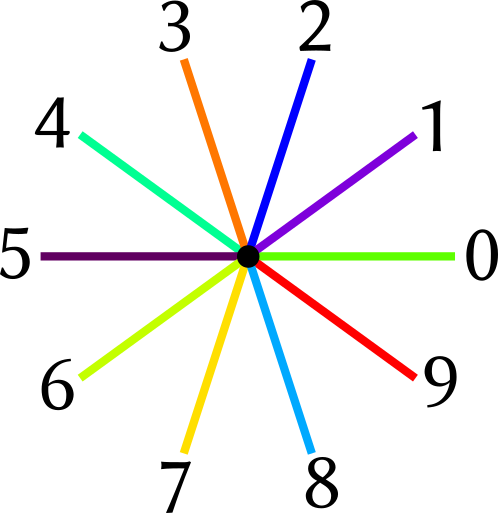
\includegraphics[width=.3\textwidth]{./bilder/kreis.png}
\end{center}
\newpage
